\chapter{Environnement de travail}
\label{sec:EnvironnementDeTravail}
Durant la réalisation de ce projet, nous avons essayé d’utiliser différents
outils de développement, d’une part afin de rendre la tâche de la
réalisation plus facile, d’autre part pour que notre système soit robuste et
répond parfaitement a nos besoins , et que nos interfaces soient claires et
faciles à utiliser.
%\section{Gestion du projet}
%Cette section est pour la présentation de mé-stratégie de fonctionnement et le programme de gestion de projets que j'ai utilisé pour lancer, structurer et gérer le travail sur ma solution.
\section{Conception}
Dans cette section, je présente le langage et le logiciel de modélisation que j’ai utilisé pour concevoir
notre solution.
\subsection{Langage de modélisation : UML}
On a utilisé UML comme langage de modélisation.
Langage de modélisation unifié UML (Unified modeling Langage) un
consiste a modéliser une application logicielle d'une façon standard
dans le cadre de conception orientée objet.
UML consiste a couvrir le cycle de vie d'un logiciel depuis la
spécification des besoins jusqu'au codage en offrant plusieurs
moyens de description et de modélisation des acteurs.
\subsection{Logiciel de modélisation} 
Visual Paradigm Online est un outil de création de diagrammes en ligne. Vous pouvez créer un nombre illimité de diagrammes, graphiques et autres visuels à partir d’un large éventail de types de diagrammes, y compris UML, organigrammes, BPMN, ERD, DFD, ArchiMate et autres.\newline\newline
%%%%%%%%%%%%%%%%%%%%%%%%%%%%%%%%%%%%%%%%%%%%%%%%%%%%%%%%% Tests %%%%%%%%%%%%%%%%%%%%%%%%%%
\begin{table}
		
	\caption{Rôles des diagrammes UML utilisés.}
	\label{table:kysymys}
\begin{tabular}{|c|p{11cm}|}
	
	\hline
	\large \bfseries Diagramme & \large \bfseries Rôle\\
	\hline
	Diagramme de cas d’utilisation & Il consiste à donner une vision globale sur les principales fonctionnalités
	(chaque fonctionnalité représente un cas d’utilisateur) d’une application .  \\
	\hline
	Diagramme d’activité &  Fournir une vue du comportement d'un système en décrivant la séquence d'actions d'un processus.    \\
	\hline
	Diagramme de séquence &Permettent d'identifier les classes requises par un système et le comportement des objets de classes au cours des interactions.  \\
	\hline
	Diagramme de classe    &Le diagramme de classes représente généralement un schéma utilisé en génie
	logiciel pour modéliser un problème bien précis, sous forme des classes et des
	interfaces ainsi que les différentes relations entre celles-ci. \\
	\hline
\end{tabular}
\end{table}
%Table \ref{table:kysymys} on page \pageref{table:kysymys} refers to the ...
\section{Implémentation}
Durant la réalisation de ce projet, nous avons essayé d’utiliser différents
outils de développement, d’une part afin de rendre la tâche de la
réalisation plus facile, d’autre part pour que notre système soit robuste et
répond parfaitement a nos besoins , et que nos interfaces soient claires et
faciles à utiliser.
\subsection{Front-end}
C’est le développement coté client autrement dit la
partie du code reçu par le client. On rappelle que le client désigne
un navigateur web.
On a choisi Flutter comme Framework pour développer la partie
front de notre application mobile.
Flutter est un framework de développement d’applications mobiles open source de Google. La principale raison de sa popularité est qu’il prend en charge la création 		   
d’applications multiplateformes. Flutter est également utilisé pour créer des apps interactives qui s’exécutent sur des pages web ou sur le bureau.
\subsubsection{Editeur de texte : VS Code}
VS Code (Visual Studio Code) est un éditeur de code source réalisé par Microsoft pour Win-
dows, Linux et macOS. [9] Les fonctionnalités incluent la prise en charge du débogage, lacoloration
syntaxique, la saisie semi-automatique intelligente du code, les extraits de code, la refactorisation du
code et Gitintégré. Les utilisateurs peuvent modifier le thème,les raccourcis clavier,les préférences et
installer des extensions qui ajoutent des fonctionnalités supplémentaires.\newline Pour en savoir plus, veillez
visiter le lien : \href{https://en.wikipedia.org/wiki/VisualStudioCode}{https://en.wikipedia.org/wiki/VisualStudioCode}
\subsubsection{Language : Dart}
Dart est un langage de programmation open source à usage général. Il est initialement développé par Google. Dart est un langage orienté objet avec une syntaxe de C-style. Il prend en chargent les concepts de programmation tels que les interfaces, les classes, contrairement aux autres langages de programmation, Dart ne prend pas en charge les tableaux.
Les collections Dart peuvent être utilisées pour répliquer des structures de données telles que des tableaux, des génériques et un typage facultatif.
\newline Pour en savoir plus, veillez
visiter le lien : \href{https://www.tutorialspoint.com/flutter/flutter_introduction_to_dart_programming.htm}{https://www.tutorialspoint.com/flutter/dart}
\subsubsection{Framework : Flutter}
Flutter est un framework de développement d’applications mobiles open source de Google. La principale raison de sa popularité est qu’il prend en charge la création 		   
d’applications multiplateformes. Flutter est également utilisé pour créer des apps interactives qui s’exécutent sur des pages web ou sur le bureau.\newline
\textbf {- Les caractéristiques de Flutter :}

\begin{enumerate}
	\item Base de code unique pour Android et iOS
	\item Fonction de rechargement à chaud (hot reload)
	\item Open-source et par Google
	\item Programmation Dart \newline \newline \newline
\end{enumerate}

\textbf {- Architecture d’une application Flutter :}\newline \newline \newline
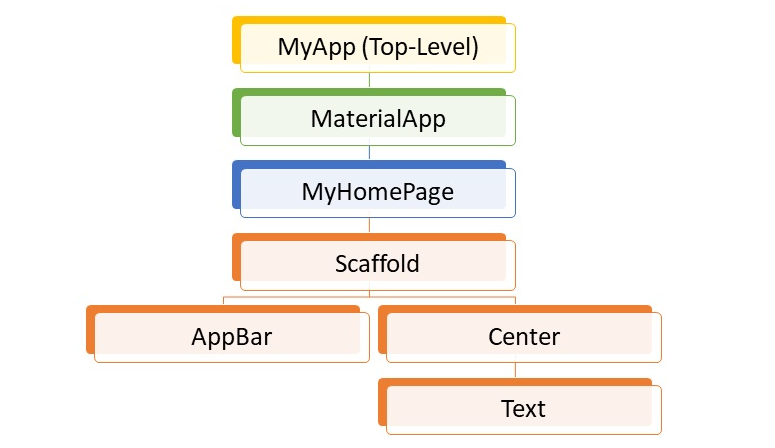
\includegraphics[width=400px,height=200px]{./Template LaTeX/Images/Flutter_architect.png}
\subsubsection{IDE : Android Studio}
Android Studio est un environnement de développement pour développer des applications mobiles Android. Il est basé sur IntelliJ IDEA et utilise le moteur de production Gradle. Il peut être téléchargé sous les systèmes d'exploitation Windows, macOS, Chrome OS et Linux.
\newline Pour en savoir plus, veillez
visiter le lien : \href{https://en.wikipedia.org/wiki/AndroidStudio.}{https://en.wikipedia.org/wiki/AndroidStudio.}
\subsection{Back-End}
C’est le développement cote serveur c’est-à-dire la partie du code exécutée par le serveur.
\subsubsection{Language : PHP}
PHP est un langage de script utilisé le plus souvent côté serveur : dans cette architecture, le serveur interprète le code PHP des pages web demandées et génère du code (HTML, XHTML, CSS par exemple) et des données (JPEG, GIF, PNG par exemple) pouvant être interprétés et rendus par un navigateur web. PHP peut également générer d'autres formats comme le WML, le SVG et le PDF.

Il a été conçu pour permettre la création d'applications dynamiques, le plus souvent développées pour le Web. PHP est le plus souvent couplé à un serveur Apache bien qu'il puisse être installé sur la plupart des serveurs HTTP tels que IIS ou nginx. Ce couplage permet de récupérer des informations issues d'une base de données, d'un système de fichiers (contenu de fichiers et de l'arborescence) ou plus simplement des données envoyées par le navigateur afin d'être interprétées ou stockées pour une utilisation ultérieure.
\newline Pour en savoir plus, veillez
visiter le lien : \href{https://fr.wikipedia.org/wiki/PHP}{https://fr.wikipedia.org/wiki/PHP}

\subsubsection{Serveur Web : Amazon Web Services (AWS)}
Amazon Web Services (AWS) est la plateforme cloud la plus complète et la plus largement adoptée au monde. Elle propose plus de 200 services complets issus de centres de données du monde entier. Des millions de clients (dont certaines des startups les plus dynamiques au monde, de très grandes entreprises et des agences fédérales de premier plan) utilisent AWS pour réduire leurs coûts, gagner en agilité et innover plus rapidement.
\newline Pour en savoir plus, veillez
visiter le lien : \href{https://aws.amazon.com/fr/what-is-aws/#:~:text=Amazon%20Web%20Services%20(AWS)%20est,de%20donn%C3%A9es%20du%20monde%20entier.}{https://aws.amazon.com/fr/what-is-aws}

\subsubsection{Framework :Laravel}
Laravel est un framework web open-source écrit en  \href{https://fr.wikipedia.org/wiki/PHP}{PHP} respectant le principe modèle-vue-contrôleur et entièrement développé en programmation orientée objet. Laravel est distribué sous \href{https://fr.wikipedia.org/wiki/Licence_MIT}{licence MIT}, avec ses sources hébergées sur 
\href{https://fr.wikipedia.org/wiki/GitHub}{GitHub}.
\subsubsection{SGBD MariaDB}
Un gestionnaire de base de données libre.
ce projet est assurée par la fondation Maria DB, et sa
maintenance par la société Monty Program AB, créateur du
projet, il confère au logiciel l'assurance de rester libre. MariaDB a
plusieurs et différentes versions. Ells s'articulent sur le code
source de MySQL de la version 5.1 aux versions plus récentes
(comme la 5.6 fin 2012). Un serveur qui stocke les données dans
des tables séparées plutôt que de tout rassembler dans une seule
table. Du coup il améliore la rapidité et la souplesse de
l'ensemble.
\subsection{Motifs d’architecture logicielle}
\subsubsection{MVC}
Le patron de conception MVC est l’une des bases du Framework
laravel, c’est-à-dire modèle-vue- contrôleur. L’interaction avec la
base de données est assurée par le Model, les regroupe, traite et
gère les données.
Pour faire afficher ce que le modèle renvoie on fait appelle a la vue .
elle s’occupe d’autre part de la réception de toute interaction de
l’utilisateur. Ce sont ces actions-là que le contrôleur gère.
Ainsi que l’échange entre le modèle et la vue. Il intercepte toutes les
activités de utilisateur et, en fonction de ces activités, il actionne les
changements à effectuer sur l'application.
Les composants sont séparés en ces trois catégories précédentes
permet une clarté de architecture des dossiers et simplifie
grandement la tâche aux développeurs.
\begin{figure}[h!]
	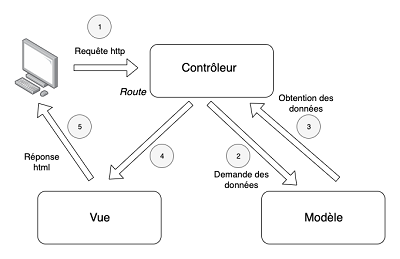
\includegraphics[width=15cm, height=8cm]{./Template LaTeX/Images/Modèle-vue-contrôleur_(MVC)_-_fr.png}
	\caption{MVC}
	\label{fig:birds}
\end{figure}
\newline \newline \newline
\textbf{Les fichiers sont organisés comme suit :}
\begin{enumerate}
	\item [-] \textbf{Route (Dispatcher) : }il contient les définitions des chemins d’entrées pour l’utilisateur,
	autrement dit les URI possibles et les dirige sur la classe définit dans
	le contrôleur qui doit traiter l’information.
	\item [-] \textbf{ Modèle : }pour chaque table de notre base de données que l’on veut
	utiliser pour notre application, il faut créer un modèle pour chacun.
	Ainsi nous avons ici un modèle de notre application. Il permet de
	décrire la méthode d’accès aux données de la base, tous cela à
	travers un objet définit par ORM Eloquent(Object-Relational
	Mapping).
	\item [-] \textbf{Contrôleur : } il permet de récupérer les informations du modèle et de l’envoyer
	vers la vue pour la mise en forme.
	\item [-] \textbf{Vue : } la vue réceptionne la réponse qui est envoyée par le
	contrôleur .\newline
\end{enumerate}
Ce figure ci-dessous résume en quelque sort le fonctionnement de
notre application.
L’api est considéré comme l’intermédiaire entre la partie données
(base de données) et la partie présentation (Application mobile).
\begin{figure}[h!]
	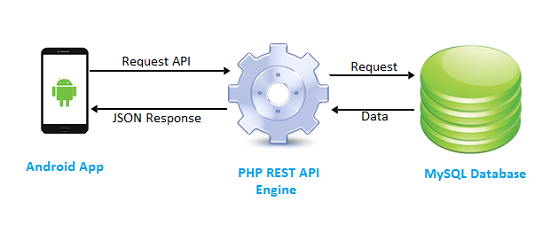
\includegraphics[width=15cm, height=8cm]{./Template LaTeX/Images/php-mysql-rest-api-for-android.png}
	\caption{PHP MySQL REST API pour Android}
	\label{fig:birds}
\end{figure}
\newline \newline \newline



